\section{Computational Structure}\label{chpt:fmm:sec:computational_structure}

Figure \ref{fig:chpt:fmm:data_flow} illustrates the dataflow in the \acrshort{fmm} when evaluating the potentials due to a set of source particles at a set of target particles in its far-field. Shown this way, it's easy to see how the spatial locality of required boxes for during the \acrshort{p2m} and \acrshort{m2m} steps during the upward pass, and the \acrshort{l2l}, \acrshort{l2p} and \acrshort{p2p} steps during the downward pass could be implemented using contiguous buffers for spatially local octant data. Indeed there are many established encodings for `space filling curves', which can be used to encode the indices of nodes in a hierarchical tree, common examples including so called Hilbert and Morton curves \cite{sagan2012space}. The power of this, in combination with an octree data structure is that it allows for extremely efficient lookups for node data, and that of nodes adjacent to a given node, as geometric information is tied to memory layout.

In terms of the tree data structure, the leaf level operators: \acrshort{l2p} \acrshort{p2m} and \acrshort{p2p} are embarrassingly parallel over each leaf. As would be the \acrshort{m2p} for an adaptive \acrshort{fmm}. In a single node setting on a \acrshort{cpu} these operators can effectively handled with a combination of multi-threading and efficient vectorisation via \acrshort{simd}, and similarly easy to translate into a \acrshort{gpu} implementation. However, in this case the small data sizes involved in the the \acrshort{l2p}, \acrshort{p2m} and \acrshort{m2p} for an adaptive \acrshort{fmm}, may make \acrshort{gpu} implementations redundant due to the memory transfer costs outweighing the increased throughput. This is enabled by the high arithmetic-intensity of leaf-level operators that involve the particle data. Consider the \acrshort{p2p}

... P2P arithmetic intensity. It is compute bound, and scales very well with direction of processor technology.

As we have seen, it is possible to form the \acrshort{m2m} and \acrshort{l2l} operators as matrix-vector products for the \acrshort{kifmm}, and also its variants [CITE FORTIN, bbFMM]. Indeed, as these operations depend on the relative position between two boxes, we can effectively block these operations as matrix-matrix products of sets of boxes at a given level, usually siblings as their coefficient data can effectively be stored contiguously in memory alongside a localtional encoding.

... Matrix multiplication is a heavily optimised routine in both software and hardware
    - BLIS, gotoblas etc.
    - special registers in Apple/new AMD/qualcomm devices due to AI

\begin{figure}[h]
    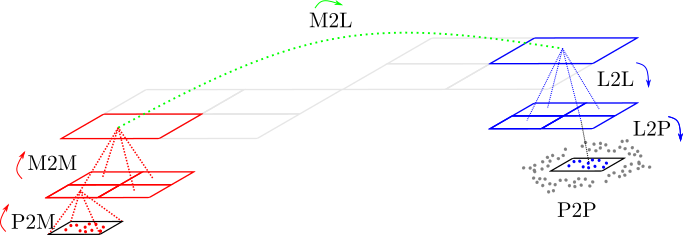
\includegraphics[width=\textwidth]{fmm_data_flow.png}
    \caption{Data flow for the evaluation of the potentials due to a given set of (red) source particles in the far field of a given set of (blue) target particles, in 2D for clarity with a uniform tree of depth 2. The source particles in the near field of the target box are shown in grey.}
    \label{fig:chpt:fmm:data_flow}
\end{figure}

However, the power of the \acrshort{fmm} and its derived asymptotic complexity come from capturing long-range interactions via the \acrshort{m2l} field translations. This naturally leads to non-contiguous memory accesses during this step, as the \acrshort{m2l} operator is only defined for non-adjacent nodes. Indeed, despite the $O(N)$ complexity, efficiently organising data for this step alone can define the runtime of a practical implementation. This is of even greater importance in 3D, where the sizes of interaction lists are larger, as well as for oscillatory problems where the rank for a given interaction grows with box diameter. Performing efficient \acrshort{m2l} requires a careful balance between efficiently handling the interaction lists to ensure contiguous data access, as well as algorithmic optimisations to reduce the complexity of this operator.

The expense of the \acrshort{fmm} can therefore be considered a trade-off between compute-bound leaf level operators, and the memory bound \acrshort{m2l} operator.

... Chandramowlishwaram result from ages ago, have things gotten worse since then for M2L?


The \acrshort{fmm} offers further opportunities for parallelism. The two most expensive parts of the \acrshort{fmm}, the \acrshort{p2p} and \acrshort{m2l} are independent from each other, and can be performed asynchronously. This is the basis of approaches which offload one of these operators, usually the \acrshort{p2p}, to a co-processor while performing the recursive loop.

Given two non-intersecting boxes at level $l$
- If their interaction lists do not overlap, they can proceed independently of one another during the downward pass
- Even if their interaction lists do overlap, if the appropriate metadata structure required for the M2L is setup - i.e. where to look for multipole data, perhaps a re-allocation to get data contiguous for lookup. They can still proceed independently of each other.
- This has remarkable consequences for parallelising distributed FMMs. Early approaches suffered from a reliance on a global all-reduce, stemming from the fact that nodes near the root are required by almost all boxes during the downward pass.
- However, as first noted by Ibeid et. al. There is (in 3D) at least an 8 fold redundancy if data is partitioned across MPI ranks such that each rank contains roots that correspond to leaves of a `global' tree.
- This means, that the FMM below the depth of the global tree, can proceed completely independently on each rank, and the communication required for the global tree is only of multipole and local coefficient data which is inherently small as only a few ranks are involved in the communication.
- The second issue in distributed memory, aside from ghost communication, is achieving an appropriate load balance among processors. This is addressed in a multitude of ways, commonly by creating a cost function that is proportional to the size of each box's interaction list, followed by a repartition of the data. As the initial partition is achieved via parallel sort, the appropriate load-balanced partition again relies on a parallel sort, for which numerous communication optimal implementations are readily available.

As we can see the most significant bottlenecks in \acrshort{fmm} implementations are related to memory transfer both vertically through the cache-hierarchy on a specific device, and horizontally among distributed devices. Specifically, the data organisation required for performing the \acrshort{m2l}, and the communication of ghost information in a distributed setting. The remainder of the algorithm can be very efficiently parallelised with established approaches, as long as care is taken to keep the computational intensity (i.e. number of effective flops) as high as possible.

The \acrshort{fmm} also exposes significant opportunities for deployment via asynchronous execution and task based runtimes, as the most time consuming sections of the algorithm can be evaluated independently of each other. Additionally, during the recursive loop, as long as appropriate metadata is created, all operations are trivially parallel over each box at a given level.

